\documentclass{cekarticle}
\usepackage{color}
\usepackage{amsmath}
\usepackage{amssymb}
\usepackage{array}

\begin{document}

%=============================================================================
% Title page
%=============================================================================

\title{Systems Biology Markup Language (SBML) Level 3 Proposal: Multi-component Species Features}

\author{Andrew Finney}

\authoremail{
\begin{minipage}{\textwidth}\centering
afinney@cds.caltech.edu
\end{minipage}}

\maketitlepage

\section{Executive Summary}
\label{Executive Summary}

%=============================================================================
\section{Terms of Reference}
\label{sec:t-o-r}
%=============================================================================

This document describes proposed features for inclusion in
Systems Biology Markup Language (SBML) Level 3. This document
describes features enabling the description of large chemical entities that are formed
from small chemical entities.  (Entities of this type were previously classed as 'complex species'.
This term is confusing~\citep{phair:2003} and is avoided in this document.)  

This document is not a definition of SBML Level 3 or part of it.
This document simply presents various features which could be
incorporated into SBML Level 3 as the Systems Biology community
wishes.  This document is intended for detailed review by that
community and to provoke alternative proposals.  

This document is not the first proposal to support multi-component species~\citep{lenovere:2002} and supersedes
a previous proposal by the author~\citep{finney:2001f}.

Throughout this
document issues that the author believes will require further
discussion have been highlighted.

For brevity the text of this document is with reference to SBML
Level 2~\citep{finney:2002f} i.e. features are described in terms
of changes to SBML Level 2.  In addition for brevity the UML diagrams in this proposal
show only new attributes and types for SBML Level 3.  

All types proposed in this document will be derived from the
\texttt{SBase} type.


\section{Acknowledgements}

This proposal has benefitted from discussions the author had with Nicolas Le Novere,
Fabian Campagne, Jeremy Zucker, Robert Phair, Larry Lok, Michael Blinov and Roger Brent.
In particular many of the ideas presented here are similar to those developed by the Molecular
Sciences Institute and the T-10 Cell Signalling Group~\citep{goldstein:2001} at Los
Alamos National Laboratories.

\section{Aims}

This proposal aims to support the representation of the following concepts that are not easily
represented in SBML Level 2:

\begin{itemize}
\item the common description of biochemical entities that can then be located in different
compartments
\item the common description of biochemical reactions that can then be located in different
compartments
\item the hierarchical description of biochemical entities through the composition of other
biochemical entities
\item the description of biochemical entities through simple associative composition
\item the description of biochemical entities through graphs of other biochemical entities
where arcs represent kinds of bonding
\item the description of generalized biochemical reactions that avoids the enumeration of
many species states and reactions
\end{itemize}

In particular this proposal aims to enable the description of, for example, proteins which
can contain many phosphorylation states,
complexes of these proteins and models of signalling pathways which contain these proteins.

\section{Overview of Proposal}

A UML diagram for the proposed new classes is shown in
figure~\ref{fig:multi-component-species-uml}.
These classes are defined in detail in section~\ref{sec:definitions}.
Section~\ref{sec:definitions} can be considered as a reference section and some readers may wish
to skip it.

Sections~\ref{sec:commonspecies} through~\ref{sec:generalizedreactions}
demonstrate with examples how the described classes can be assembled to
achieve the aims of the proposal.  These section effectively define a roadmap
of how the feature described in this proposal could be added in to SBML in stages.

\begin{figure}[h]
  \vspace*{8pt}
  \centering
  \includegraphics[scale = 0.7]{multi-component-species.eps}
  \caption{The types and attributes introduced into SBML by this proposal.  This diagram
  only shows new classes and fields: all SBML Level 2 structures are assumed to be present.}
  \label{fig:multi-component-species-uml}
\end{figure}

\section{Proposed Classes in Detail}
\label{sec:definitions}
This section describes in detail each class in the proposal as shown in
figure~\ref{fig:multi-component-species-uml}.
As in the diagram only new or extended classes are described in this section.
All level 2 structures are assumed to be present.
For each new or extended class the definition of the class and its fields are described.

\attrib{id} fields on structures, described here, enclosed within a \class{SpeciesType} structure
are unique to that structure only.
\attrib{id} fields on structures, described here, enclosed within a \class{Reaction} structure are
unique to that reaction only (apart from the \attrib{id} fields of \class{SimpleSpeciesReferences}
which are unique to a whole model).

The definition of \class{species} and \class{speciesType} may not be as one would
expect in conventional biochemical terminology because \class{species} retains its definition
from SBML Level 1 and 2.

\subsection{Bond}

The abstract base class \class{Bond} represents one or more chemical bonds or forces holding two chemical
entities together enabling them to form a larger chemical entity.  A \class{bond} can represent
covalent and non-covalent bonds.  The existence of a \class{bond} can imply some
modification of the chemical entities.  For example a phosphorylated protein can be represented
in a model as a \class{bond} between a protein and a phosphate group.  In such a model
the loss of the hydrogen atom bound to the phosphorylation site may or may not be represented
explicitly and does not affect the identity of the protein.  

A \class{Bond} structure consists of one \class{BindingSiteReference} field,
\attrib{bindingSite}, which indicates where the bond has effect.

The linkage of chemical entities together to form a larger chemical entity can be 
represented without using \class{bonds}.  See section~\ref{sec:multicomponentspecies}.

\subsection{BindingSite}

A logical site where a bond may form on the chemical entity represented by the
enclosing \class{SpeciesType} structure.  A \class{BindingSite} may represent a set of
physical binding sites which are treated as a single entity for the purposes of the model.  
A \class{BindingSite} structure consists of

\begin{itemize}

\item \attrib{id}, a mandatory \class{SId} field to identify the site

\item \attrib{name}, an optional string field (see SBML Level 2)

\item \attrib{bindingSiteReference}, an optional field containing a
\class{BindingSiteReference} structure.  When this attribute is present the binding site is
exposing an internal binding site on a \class{SpeciesTypeInstance}.
\attrib{bindingSiteReference} refers to a binding site internal to the enclosing
\class{SpeciesType} which is not referenced by another \attrib{bindSiteReference}.

\end{itemize}

\subsection{BindingSiteReference}

A reference to an instance of a \class{BindingSite} in a given \class{SpeciesGraph}.
A \class{BindingSiteReference} structure consists of

\begin{itemize}

\item \attrib{speciesTypeInstance}, a \class{SId} field,
which refers to a \class{SpeciesTypeInstance} within the enclosing
\class{SpeciesGraph}; and

\item \attrib{bindingSite}, a \class{SId} field, which refers to a \class{binding site}
on that instance (declared on the \class{SpeciesType} referenced by the
\class{SpeciesTypeInstance}).

\end{itemize}

The combination of attribute values of a given \class{BindingSiteReference} structure cannot
occur in any other \class{BindingSiteReference} structure within the same \class{SpeciesGraph}
structure.  

\subsection{GenericBond}

Represents a chemical bond between a specific binding site and an unspecified chemical entity.
\class{GenericBond} is a subtype of \class{Bond}.  \class{GenericBond} consists
of two fields: \attrib{bindingSite}, a \class{BindingSiteReference} structure inherited from
\class{Bond} and \attrib{subGraph}, a class{SId} field which refers to an unspecified
chemical entity.

\class{GenericBond} structures can only occur within \class{Reactions}. (They can only occur
in the \class{bond} array/list field in \class{SimpleSpeciesReference}.)

The values of \attrib{subGraph} fields are specific to one reaction.  All \attrib{subGraph}
fields with the same value in the same reaction refer to the same chemical entity.
\attrib{subGraph} fields in different reactions refer to different chemical entities.
\attrib{subGraph} fields with different values refer to different chemical entities.

\subsection{Model}

See SBML Level 2 for the existing definition of \class{model}.  This proposal adds a
\attrib{speciesType} field which consists of a list of \class{SpeciesType} structures to
\class{Model} structures.  

This proposal changes the definition of the \attrib{species} list on \class{model}.
This list does not necessarily comprise the complete set of pools of chemical entities in the model.
The set of \class{Species} structures in this list which have an undefined or non-zero
initial amount or concentration, \emph{initial species}, are used to infer the complete set
of pools of chemical entities in the model.  The complete set of species located in a given
compartment can be inferred by traversing the reaction
network, defined by the set of \class{Reaction}, from the initial species that are located in
the compartment.

\subsection{Reaction}

A reaction
is either located inside a specific compartment, across more than 2 or more compartments or
 potentially in all compartments.  This final case is indicated by the absence of 
\attrib{compartment} and \attrib{species} fields on all enclosed \class{SimpleSpeciesReference}
structures. In this case the \class{SimpleSpeciesReference} structures match with \class{Species}
in the same \class{Compartment} across all compartments in the model.
See section~\ref{sec:commonreaction}

\subsection{SimpleSpeciesReference}

See SBML Level 2 for the existing definition of \class{SimpleSpeciesReference}.
\class{SimpleSpeciesReference} is the base class for: (a) \class{SpeciesReference} the type used
to represent the reactants and products of a reaction and (b) \class{ModifierSpeciesReference} the
type used to represent the modifiers of a reaction.  \class{SimpleSpeciesReference} structures
can only occur within a reaction.

In this proposal a \class{SimpleSpeciesReference} can refer to a set of \class{Species} both
those that are explicitly defined and those that are created through generalized reactions
(see section~\ref{sec:generalizedreactions}).  (A \class{SimpleSpeciesReference} on its own does not
imply the existence of a \class{Species}.)

In this proposal a \class{SimpleSpeciesReference} becomes a subtype of \class{SpeciesGraph}.

\class{SimpleSpeciesReference} has the following fields:

\begin{itemize}

\item \attrib{id}, this optional \class{SId} field is not introduced by this proposal but instead
it has a new role: the value of this field can be used as a symbol, enclosed in MathML\texttt{ci}
elements, within the \class{KineticLaw} structure of the enclosing \class{Reaction} structure.

\item \attrib{substanceUnits}, \attrib{spatialSizeUnits} and \attrib{hasOnlySubstanceUnits},
these optional fields have the same semantics as the corresponding attributes on \class{Species}.
These attributes default to the values of matching \class{Species} structures before following the
\class{Species} semnatics.
\class{SimpleSpeciesReference} structures that match with a \class{Species} structure should
default to the \class{Species} attributes and/or be exactly equivalent to them.  Two 
\class{SimpleSpecisReference} structures that refer to the same inferred species should have
the same units.

\item \attrib{species}, this \class{SId} field is present in Level 2 however we now make this field
optional.  This field refers to a \class{Species} that is involved in the reaction.  If this field is
present then the fields inherited from \class{SpeciesGraph} as well as the \attrib{compartment},
\attrib{bond} and \attrib{speciesType} fields are not available.

\item \class{speciesType}, this \class{SId} field refers to a \class{SpeciesType} that is
involved in the reaction.  If this field is
present then the fields inherited from \class{SpeciesGraph} as well as the 
\attrib{Species} and \attrib{bond} fields are not available.  If the \class{compartment}
field is present then the \class{SimpleSpeciesReference} refers to the \class{Species} of
the given \class{SpeciesType} located in the given \class{compartment}; otherwise the
\class{SimpleSpeciesReference} refers to a set of \class{Species} of the given \class{SpeciesType}.

\item \class{compartment}, this \class{SId} field refers to a \class{Compartment} where the matching
\class{Species} are located.  If this field is not present a given \class{SimpleSpeciesReference}
structure then it must not be present on any other 
\class{SimpleSpeciesReference} structure in the same enclosing \class{reaction}.

\end{itemize}

\subsection{Species}
\label{sec:species}

See SBML Level 2 for the existing definition of \class{Species}.  In this proposal a 
\class{Species} structure represents a pool of a given chemical entity located in a specific
compartment. 
This proposal introduces one optional \class{SId} field, \attrib{speciesType} which refers to
the \class{SpeciesType} (chemical entity) to be located in the \class{Compartment} referenced by
the \attrib{compartment} field.  There can only one \class{Species} structure in a model with a given
pair of values for the \attrib{speciesType} and \attrib{compartment} attributes i.e.
a given \class{SpeciesType} cannot be located in the same \attrib{Compartment} mode than once.

\emph{revise this:}
When the \attrib{speciesType} field is not present then the \class{Species} structure is equivalent
to a \class{Species} structure which does contain a \attrib{speciesType} field.
This field would refer to a \class{SpeciesType} that is not referenced anywhere else in the model.
In short a \class{Species} structure without a \attrib{speciesType} field has a
`hidden' \class{SpeciesType} associated with it.

\subsection{SpeciesGraph}

\class{SpeciesGraph} is an abstract base class.
A \class{SpeciesGraph} structure represents a chemical entity or a set of chemical entities of
a specific common form.  The form of these entities is defined as a graph where the nodes are
\class{SpeciesTypeInstances} and the arcs are \class{Bond} structures.  The graph can be disconnected
indicating that the detail of how parts of the chemical entities are associated are not relevant to the
model (see~\ref{sec:multicomponentspecies}).  

A \class{SpeciesGraph} structure is composed of the following fields:

\begin{itemize}

\item \attrib{speciesTypeInstance}, this is an optional list of \class{SpeciesTypeInstance}
structures that the \class{SpeciesGraph} is composed from.  If this list is not present
then the \class{SpeciesGraph} simply represents an chemical entity for which the detail
of its composition is not relevant to the model.

\item \attrib{unboundSite}, this is an optional list of \class{BindingSiteReference} structures which
refer to the binding sites on the \class{SpeciesTypeInstance} structures in the \class{SpeciesGraph}
which are unbound (not part of a \class{Bond}).  In model an unbound binding site may have
some implied chemical structure which is not made explicit i.e. the binding site may not be physically
unoccupied and the entity occupying the site is simply not modelled.

\item \class{bond}, an optional list of \class{Bond} structures that link the chemical entities 
enumerated in the \attrib{speciesTypeInstance} field inherited from \class{SpeciesGraph}.
This list can include both \class{SpecificBond} and \class{GenericBond} structures.

\end{itemize}

\subsection{SpeciesType}

The class \class{SpeciesType} is derived from \class{SpeciesGraph} and represents a specific
chemical entity.  A \class{SpeciesType} structure has the following fields:

\begin{itemize}

\item \attrib{id} a mandatary \class{SId} field that identifies the \class{SpeciesType}

\item \attrib{name}, an optional string field (see SBML Level 2)

\item \attrib{bindingSite}, an optional \class{BindingSite} list, which contains the set of binding
sites that are located on the \class{SpeciesType}.

\end{itemize} 

A simple example of the use \class{SpeciesType} structures is given in section~\ref{sec:commonspecies}.

\subsection{SpeciesTypeInstance}

A \class{SpeciesTypeInstance} structure represents the occurrence of a chemical entity of a given
\class{SpeciesType} within a \class{SpeciesGraph}.  A \class{SpeciesTypeInstance} structure has the
following fields:

\begin{itemize}

\item \attrib{id} a mandatory \class{SId} field that identifies the \class{SpeciesTypeInstance}.
This field is unique to the enclosing \class{SpeciesGraph} structure and the enclosing
\class{Reaction} structure if it exists.

\item \attrib{name}, an optional string field (see SBML Level 2)

\item \attrib{speciesType}, a mandatory \class{SId} field which refers to the \class{SpeciesType}
that the \class{SpeciesTypeInstance} is an instance of.

\end{itemize}

\subsection{SpecificBond}

A subtype of \class{Bond}.   \class{SpecificBond} represents one or more chemical bonds between
two explicitly identified binding sites.  A \class{bond} structure consists of two
\class{bindingSiteReference} structures,
\attrib{bindingSite} (inherited from \class{Bond}) and
\attrib{otherBindingSite}.
These fields which represent the 2 binding sites that are linked by the bond.
Neither binding site has privileged semantics.
See section~\ref{sec:explicitbonds} for examples.

\section{Tutorial on the Proposed Features}

\subsection{The Definition of Chemical Entities across Compartments}
\label{sec:commonspecies}

Consider a model where we have a chemical entity which exists in more than one compartment.
for example we might wish to model Aspartate in a Cytosol compartment and in the Mitochondrial Matrix.
In SBML Level 2 we have represent each pool of Aspartate located in a separate compartment, using a
\class{Species} structure:

\begin{example}
<model id="malate_aspartate_shuttle1">
    <listOfCompartments>
        <compartment id="Cytosol"/>
        <compartment id="Mitochondrial_Matrix"/>
    </listOfCompartments>
    <listOfSpecies>
        <species id="Aspartate_in_Cytosol" compartment="Cytosol"/>
        <species id="Aspartate_in_Mitochondrial_Matrix" compartment="Mitochondrial_Matrix"/>
    </listOfSpecies>
</model>
\end{example}

In SBML Level 2 there is no formal way to relate these species together.  Under this proposal
we do this by representing the Aspartate with a \class{SpeciesType} structure and then
referring to the \class{SpeciesType} from the \class{Species} structures.  We can thus transform the 
above example to:

\begin{example}
<model id="malate_aspartate_shuttle2">
    <listOfCompartments>
        <compartment id="Cytosol"/>
        <compartment id="Mitochondrial_Matrix"/>
    </listOfCompartments>
    <listOfSpeciesTypes>
        <speciesType id="Aspartate"/>
    </listOfSpeciesTypes>
    <listOfSpecies>
        <species
            id="Aspartate_in_Cytosol"
            speciesType="Aspartate"
            compartment="Cytosol"/>
        <species
            id="Aspartate_in_Mitochondrial_Matrix"
            speciesType="Aspartate"
            compartment="Mitochondrial_Matrix"/>
    </listOfSpecies>
</model>
\end{example}

This model does not introduce any new variables that are not present in
\texttt{malate\_aspartate\_shuttle1} it simply identifies \texttt{Aspartate\_in\_Cytosol}
and \texttt{Aspartate\_in\_Mitochondrial\_Matrix} as being separate pools of the same chemical entity.
You cannot refer to \class{SpeciesType} structures from MathML structures under this proposal.

The \texttt{malate\_aspartate\_shuttle1} example is still a valid model under this proposal.
For backwards compatibility the \attrib{speciesType} attribute on \class{Species} is not
mandatory.

It is not possible to locate a \class{SpeciesType} in a \class{Compartment} more than once
i.e. it is not possible for two \class{Species} structures to have the same
\attrib{speciesType} and \attrib{compartment} values.

\subsection{Generalized Reactions: The Definition of Reactions across Compartments}
\label{sec:commonreaction}

Just as we would wish to give a common identify to chemical entities distributed across several
compartments we would wish to have some common object describing reactions between those chemical
entities that is independent of the compartments in which the reactions occur.

For example consider the representation of the transamination reaction, a reversible reaction
that converts Aspartate to Oxaloacetate in both the Cytosol and Mitochondrial Matrix.

we could extend \texttt{malate\_aspartate\_shuttle2} using the SBML Level 2 form:
\begin{example}
<model id="malate_aspartate_shuttle3">
    <listOfCompartments>
        <compartment id="Cytosol"/>
        <compartment id="Mitochondrial_Matrix"/>
    </listOfCompartments>
    <listOfSpeciesTypes>
        <speciesType id="Aspartate"/>
        <speciesType id="Oxaloacetate"/>
    </listOfSpeciesTypes>
    <listOfSpecies>
        <species
            id="Aspartate_in_Cytosol"
            speciesType="Aspartate"
            compartment="Cytosol"/>
        <species
            id="Aspartate_in_Mitochondrial_Matrix"
            speciesType="Aspartate"
            compartment="Mitochondrial_Matrix"/>
        <species
            id="Oxaloacetate_in_Cytosol"
            speciesType="Oxaloacetate"
            compartment="Cytosol"/>
        <species
            id="Oxaloacetate_in_Mitochondrial_Matrix"
            speciesType="Oxaloacetate"
            compartment="Mitochondrial_Matrix"/>
    </listOfSpecies>
    <listOfReactions>
        <reaction id="Transamination_in_Cytosol" reversible="true">
            <listOfReactants>
                <speciesReference species="Aspartate_in_Cytosol"/>
            </listOfReactants>
            <listOfProducts>
                <speciesReference species="Oxaloacetate_in_Cytosol"/>
            </listOfProducts>
        </reaction>
        <reaction id="Transamination_in_Mitochondrial_Matrix" reversible="true">
            <listOfReactants>
                <speciesReference species="Aspartate_in_Mitochondrial_Matrix"/>
            </listOfReactants>
            <listOfProducts>
                <speciesReference species="Oxaloacetate_in_Mitochondrial_Matrix"/>
            </listOfProducts>
        </reaction>
    </listOfReactions>
</model>
\end{example}

Under this proposal we can replace the 2 reactions above with a single reaction structure:

\begin{example}
<model id="malate_aspartate_shuttle4">
    <listOfCompartments>
        <compartment id="Cytosol"/>
        <compartment id="Mitochondrial_Matrix"/>
    </listOfCompartments>
    <listOfSpeciesTypes>
        <speciesType id="Aspartate"/>
        <speciesType id="Oxaloacetate"/>
    </listOfSpeciesTypes>
    <listOfSpecies>
        <species
            id="Aspartate_in_Cytosol"
            speciesType="Aspartate"
            compartment="Cytosol"/>
        <species
            id="Aspartate_in_Mitochondrial_Matrix"
            speciesType="Aspartate"
            compartment="Mitochondrial_Matrix"/>
        <species
            id="Oxaloacetate_in_Cytosol"
            speciesType="Oxaloacetate"
            compartment="Cytosol"/>
        <species
            id="Oxaloacetate_in_Mitochondrial_Matrix"
            speciesType="Oxaloacetate"
            compartment="Mitochondrial_Matrix"/>
    </listOfSpecies>
    <listOfReactions>
        <reaction id="Transamination" reversible="true">
            <listOfReactants>
                <speciesReference speciesType="Aspartate"/>
            </listOfReactants>
            <listOfProducts>
                <speciesReference speciesType="Oxaloacetate"/>
            </listOfProducts>
        </reaction>
    </listOfReactions>
</model>
\end{example}

The reaction structure represents the set of reactions which occurs in all compartments where 
the reactant or product are located.  This reaction would only occur where the reactant is located
if the reaction was not reversible.  All the \class{SimpleSpeciesReference} structures refer to 
species in the same compartment.  This means that, under this proposal, it is not possible to define
a transport reaction, that is a reaction which moves chemical entities between compartments,
using this simple form.  However a variant form is described in
section~\ref{sec:locatedspeciesreferences} which employs a similar form to transport reactions.

\subsubsection{Defining the explicit location of a \class{SimpleSpeciesReference}}
\label{sec:locatedspeciesreferences}

The location of a species pool can be made explicit in a \class{SimpleSpeciesReference} structure
without referring to a \class{Species} structure.  This can be achieved by using the proposed optional
\attrib{compartment} field which refers to a \class{Compartment} structure to indicate the 
location of the given \class{SpeciesType}.

For example consider the following transport reaction that can be added to model
\texttt{malate\_aspartate\_shuttle4}:

\begin{example}
<reaction id="Malate_Transport" reversible="false">
    <listOfReactants>
        <speciesReference speciesType="Malate" compartment="Cytosol"/>
    </listOfReactants>
    <listOfProducts>
        <speciesReference speciesType="Malate" compartment="Mitochondrial_Matrix"/>
    </listOfProducts>
</reaction>
\end{example}

\emph{This feature could be introduced later in the SBML development road map.
It is however an essential component of features introduced later.}

All the \class{SimpleSpeciesReference} structures of a reaction should simultaneously either
(a) be located (i.e. have values for the \attrib{species} or \attrib{compartment} attributes);
or (b) apply to any compartment (i.e. not have values for the \attrib{species} and \attrib{compartment}
attributes). \emph{This restriction is not essential but simplifies the interpretation of
the proposed format}.

\subsubsection{Defining Kinetic Laws for Generalized Reactions}

As defined in the examples above it is not possible to compose the kinetic law of these generalized
reactions since there is no symbol that refers to either the modifiers, reactants or products or the
reaction species pools.  However under this proposal the \attrib{id} field of a
\class{SimpleSpeciesReference} becomes a symbol that can be used in the \class{KineticLaw} of the 
enclosing \class{Reaction}.

\emph{Here I am assuming that the \attrib{id} field on \class{SimpleSpeciesReference} is introduced by a
new version of SBML Level 2 as proposed by ??? in ???. This \attrib{id} field is in the global symbol
namespace despite, for the purposes of this proposal, only having scope in the enclosing
\class{Reaction}.  If this is problematic then perhaps we could consider an additional attribute to
declare the \class{symbol}.}

As example here is the \texttt{Transamination} reaction, from model
\texttt{malate\_aspartate\_shuttle4}, modified to include a rate law:

\begin{example}
<reaction id="Transamination" reversible="true">
    <listOfReactants>
        <speciesReference id="S1" speciesType="Aspartate"/>
    </listOfReactants>
    <listOfProducts>
        <speciesReference speciesType="Oxaloacetate"/>
    </listOfProducts>
    <kineticLaw>
        <math xmlns="http://www.w3.org/1998/MathMathML">
            <apply>
                <times/>
                <cn>1.1</cn>
                <ci>S1</ci>
            </apply> 
        </math>
    </kineticLaw>
</reaction>
\end{example}

\subsubsection{The Unit Attributes of \class{SimpleSpeciesReference}}

To make the units of species explicit in kinetic laws under this proposal 
\class{SimpleSpeciesReference} structures have the attributes \attrib{substanceUnits},
\attrib{spatialSizeUnits} and \attrib{hasOnlySubstanceUnits}.  These have the same semantics as
the corresponding attributes on \class{Species}.  The unit attributes of a
\class{SimpleSpeciesReference} structure that match with a \class{Species} structure should
default to the \class{Species} attributes and/or be exactly equivalent to them.  

EXAMPLE HERE

\subsection{Inferring Species}

Under this proposal \class{Species} structures are used to indicate the initial conditions
and/or attributes of specific pools of chemical entities (species) and don't represent the complete
set of pools.  In SBML Level 2 the model's \attrib{species} list is a complete enumeration of the
pools of chemical entities.  Instead, in this proposal, the set of \class{Species} structures
which have an undefined or non-zero initial amount or concentration, \emph{initial species}, are used 
as a starting point to infer the complete set of species in the model.  The complete set of species
located in a given compartment can be inferred by traversing the reaction
network, defined by the set of \class{Reaction} structures, from the initial species that are located
in the compartment.

So if we consider the model \texttt{malate\_aspartate\_shuttle4} the existence of
\texttt{Oxaloacetate} in the compartment \texttt{Cytosol} can be inferred given the reaction
\texttt{Transamination} and the species \texttt{Aspartate\_in\_Cytosol}.  This means we can omit
the species \texttt{Oxaloacetate\_in\_Cytosol} from the model as follows

\begin{example}
<model id="malate_aspartate_shuttle5">
    <listOfCompartments>
        <compartment id="Cytosol"/>
        <compartment id="Mitochondrial_Matrix"/>
    </listOfCompartments>
    <listOfSpeciesTypes>
        <speciesType id="Aspartate"/>
        <speciesType id="Oxaloacetate"/>
    </listOfSpeciesTypes>
    <listOfSpecies>
        <species
            id="Aspartate_in_Cytosol"
            speciesType="Aspartate"
            compartment="Cytosol"/>
        <species
            id="Aspartate_in_Mitochondrial_Matrix"
            speciesType="Aspartate"
            compartment="Mitochondrial_Matrix"/>
    </listOfSpecies>
    <listOfReactions>
        <reaction id="Transamination" reversible="true">
            <listOfReactants>
                <speciesReference speciesType="Aspartate"/>
            </listOfReactants>
            <listOfProducts>
                <speciesReference speciesType="Oxaloacetate"/>
            </listOfProducts>
        </reaction>
    </listOfReactions>
</model>
\end{example}

\emph{The inference of species could be introduced later in the SBML development road map.
It is however an essential component of features introduced later.}

Just as it is not possible to locate a \class{SpeciesType} in \class{Compartment} more than
once the process of inferring the complete set of species may start from the initial species
set and match with other \class{Species} that have for example a initial concentration of zero.
The inference process does not create duplicate species.

Inferred species, which don't match any \class{Species} structures, always have an initial
concentration or substance amount of zero and are never
constant nor boundary conditions.  This means that constant or boundary condition pools or pools
with any initial concentration must be made explicit using a \class{Species} structure.
Two 
\class{SimpleSpecisReference} structures that refer to the same inferred species should have
the same units.

\emph{The above definition implies that the units of \class{SimpleSpeciesReference} can vary
depending on the species that is being matched with.  It is open question whether this condition
is actually a problem or not}

Reactions of the form used in the example reaction \texttt{Malate\_Transport} fit in with the
inference scheme: if \texttt{Malate} exists in the
\texttt{Cytosol} then we can infer the existence of a pool of \texttt{Malate} in the
\texttt{Mitochondrial\_Matrix}.  Given this form of reaction \class{Species} structures are only
required to define the initial conditions of a model.

\subsection{Simple Multi-Component Chemical Entities}
\label{sec:multicomponentspecies}

\subsection{Multi-component Chemical Entities with explicit bonds}
\label{sec:explicitbonds}

\subsection{Reactions generalized to cover classes of Multi-component Chemical Entities}
\label{sec:generalizedreactions}

\subsubsection{Generalized Multi-component Chemical Entities}

\subsection{Hierarchal Species Types and Type Equivalence}

\section{Option - Reaction Predicates}

\section{Option - SpeciesType inheritance}

\section{Discussion - Model Composition and Multi-component Species}

\section{Discussion - reaction specificity - do we need groups?}

\section{Discussion - Attributes of Species and Species Types}

\newpage
\section{Appendix}
\setcounter{secnumdepth}{2}
\appendix

\section{Elements introduced in this proposal}
\section{Attributes introduced in this proposal}
%=============================================================================
% References
%=============================================================================

\bibliographystyle{apalike}
\bibliography{strings,a,b,c,d,e,f,g,h,i,j,k,l,m,n,o,p,q,r,s,t,u,v,w,x,y,z}
\end{document}
